\section{Задачи №4 ЕГЭ (преобразование выражений)}

% 4 1)отдельно (формулы) естественно появляется обратная задача. 2)Сослаться на Латех (MathJax) основные команды которыми пользуемся в Латехе texfrag и тп 
% тут рассказать много про MathJax
% закинуть фото ДЛЯ КАЖДОГО пункта
\subsection{Основные используемые команды}

Задачи этого вида проверяют умение подставлять значения в формулы, преобразовывать выражения (в том числе со стандартными функциями и корнями), аккуратно работать с единицами измерения и корректно представлять результат. 
В нашем генераторе текст формулировок размечается \emph{TeX}-фрагментами и рендерится через MathJax. 
При включённой опции \verb|autoLaTeX| (см. ниже) TeX-формулы можно вставлять непосредственно в строку без явного окружения \verb|$...$|.

Пример:
\begin{lstlisting}
NAtask.setTask({
			text:
				'В фирме «' + name + '» стоимость (в рублях) колодца из железобетонных колец рассчитывается по формуле $C = ' + plus + '+' + multiply + 
				' \\cdot n$, где $n$ – число колец, ' +
				'установленных при рытье колодца. ' +
				'Пользуясь этой формулой, ' +
				'рассчитайте стоимость колодца из $' + number + '$ колец.',
			answers: cost,
		});
\end{lstlisting}
\textsl{Задача №124.}

\lstinputlisting[]{code/4/124.js} 
До:

После:

\includegraphics[width=1.4\textwidth]{124-4.png}
\begin{lstlisting}
NAtask.setTask({

			text: 'Количество теплоты (в джоулях), полученное однородным телом при нагревании, ' +
				'вычисляется по формуле $Q = cm(t_2 - t_1)$, где $c$ – удельная теплоёмкость (в Дж),' +
				' $m$ – масса тела (в килограммах), $t_1$ – начальная температура тела (в кельвинах), а $t_2$' +
				' – конечная температура тела (в кельвинах). Пользуясь этой формулой, ' +
				the_orderToFind + ' $Q$ (в джоулях), если $t_2 = ' + t_2 + '$ К, $c = ' + c + '$ $\\frac{\\mbox{Дж}}{\\mbox{кг} \\cdot \\mbox{К}}$,' +
				' $m = ' + m + '$ кг и $t_1 = ' + t_1 + '$ К.',
			answers: Q,

		});
\end{lstlisting}
\textsl{Задача №509609.}

\texttt{\\frac{}{}}, \texttt{\\sqrt{}} и \texttt{\\sin{}} 
самые часто используемые LaTeХ команды и задачах вида 4, для отображения дробей,корней и sin.

Пример:
\begin{lstlisting}
NAtask.setTask({
			text: 'Радиус окружности, описанной около треугольника, ' +
				'можно вычислить по формуле $R = \\frac{a}{2\\sin{\\alpha}}$, где $a$ – сторона, ' +
				'а $\\alpha$ – противолежащий ей угол треугольника. ' +
				'Пользуясь этой формулой, ' + the_orderToFind + ' $' + ['R', 'a'][rand] + '$' +
				', если $' + ['a =' + a, 'R =' + R][rand] + '$ и $\\sin{\\alpha} = \\frac{' + num + '}{' + deNum + '}$.',
			answers: [R, a][rand],
			preference: preference,
		});
\end{lstlisting}
\textsl{Задача №506300.}

\subsection{Адаптирование команд}
Чтобы уменьшить рукописный TeX и исключить мелкие огрехи, используются вспомогательные методы форматирования. Например \texttt{.texfrac()}.
Удобная обёртка для дробей: на основе числителя/знаменателя или числового значения возвращает корректную TeX-строку вида \verb|\frac{p}{q}|. 
Метод избавляет от ручной конкатенации строк и повышает читаемость шаблона.
Пример:
\begin{lstlisting}
NAtask.setTask({

			text: 'Теорему синусов можно записать в виде  $ \\frac{a}{\\sin{\\alpha}} = \\frac{b}{\\sin{\\beta}} $' +
				', где $a$ и $b$ - две стороны треугольника, а $\\alpha$ и $\\beta$ - углы треугольника, лежащие против них соответственно. ' +
				' Пользуясь этой формулой, ' + the_orderToFind + ' ' + '$' + ['\\sin{' + nameSin[0] + '}', nameLetter[0]][rand] + '$' +
				', если ' + '$' + [nameLetter[0] + ' =' + a, '\\sin{' + nameSin[0] + '} =' + sinA.texfrac(1)][rand] + '$' +
				', $' + nameLetter[1] + ' =' + b + '$, $\\sin{' + nameSin[1] + '} = ' + sinB.texfrac(1) + '$.',
			answers: [sinA, a][rand],
			preference: preference,

		});
\end{lstlisting}
\textsl{Задача №530329.}
\lstinputlisting[]{code/4/530329.js} 
До:
После:

\includegraphics[width=1.4\textwidth]{530329-4-1.png}

\includegraphics[width=1.4\textwidth]{530329-4-2.png}

\includegraphics[width=1.4\textwidth]{530329-4-3.png}

\includegraphics[width=1.4\textwidth]{530329-4-4.png}
%Закинуть фото разницы между \\frac{}{} и texfrac() ???

 \texttt{.shuffle()} перемешивает массив (например, буквы параметров) для вариативности формулировок.

Пример:
\begin{lstlisting}
let letter = ['a', 'b', 'c'].shuffle();
\end{lstlisting}
\textsl{Задача №2939.}
\lstinputlisting[]{code/4/2939.js} 
До:
После:

\includegraphics[width=1.4\textwidth]{2939-4-1.png}

\includegraphics[width=1.4\textwidth]{2939-4-2.png}

\includegraphics[width=1.4\textwidth]{2939-4-3.png}

\texttt{.sqrt()} \texttt{.cbrt()} - утилиты для корней второй и третьей степеней. Удобны как при вычислении ответов, так и при генерации правдоподобных «отвлекающих» значений.
Так же \texttt{.rod} - определяет грамматический род существительного: \verb|0| — м.р., \verb|1| — ж.р., \verb|2| — ср.р., \verb|3| — всегда множественное. 
Это позволяет автоматически согласовать местоимения и прилагательные в задачах.
Пример:
\lstinputlisting[]{code/4/512937.js} 
До:
После:

\includegraphics[width=1.4\textwidth]{512937-4-1.png}
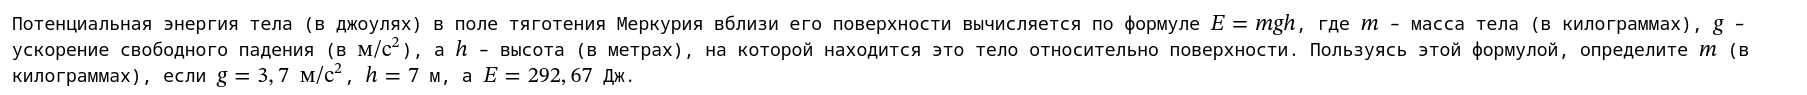
\includegraphics[width=1.4\textwidth]{512937-4-2.png}


\texttt{isValidTriangle()} - из  flatten-shape-geometry 1.8.2, из 3 переменных проверяет могут ли они составить треугольник. и выдают true - если является, и false -если нет
Пример:
\begin{lstlisting}
	let a = sl(2, 30);
		let b = sl(2, 30);
		let c = sl(2, 30);

		genAssert(isValidTriangle(a, b, c), 'Должно являться треугольником');
\end{lstlisting}
\textsl{Задача №506550.}

\texttt{.isZ()} проверка «число является целым». Удобно для отсечения случаев, в которых формула даёт «некрасивый» ответ. Чае всего используется вместе с genAssert   
Пример:
\begin{lstlisting}
let second = sl(5, 30);
		let amperage = sl(5, 30);
		let voltage = sl(5, 30);
		let resistance = slKrome([amperage, voltage, second], 5, 30);
		let answer = [amperage ** 2 * resistance * second, voltage ** 2 * second / resistance][rand];

		genAssert(answer.isZ(), 'должно быть целым');
\end{lstlisting}
\textsl{Задача №523098.}


%\prototype[separator]{Array}{shuffleJoin}
%Перемешивает и соединяет массив с разделителем \texttt{separator}. \texttt{separator} по умолчанию пустая строка. Функция используется в листинге \ref{lst:3011}
%в строке \ref{line:shuffleJoin} для отображения условий задачи в случайном порядке.
%%\begin{lstlisting}
%    let array = ['A', 'B', 'C', 'D',];
%    array.shuffleJoin();
%    //ADBC

%    array.shuffleJoin('; ');
%    //C; D; B; A 
%\end{lstlisting}

\subsection{Обратные задачи}
Многие шаблоны №4 имеют \emph{парные} (обратные) постановки: в одном варианте требуется найти, например, \(R\), в другом — \(a\), в третьем — \(\sin\alpha\) и т. п. 
Переключение таких вариантов реализовано через массив предпочтений \verb|preference| и выбор сценария. 

Пример: 
\begin{lstlisting}
let preference = ['find_R', 'find_a', 'find_sin']; // «обратные» постановки
let key = '506300';
let rand = getListedPreference(
  key,
  preference.map((pref, idx) => ({ preference: pref, preferenceValue: idx })),
  sl(preference.length - 1)
);

if (preference[rand] === 'find_R') {
  // генерируем данные так, чтобы удобно было находить R
} else if (preference[rand] === 'find_a') {
  // обратная постановка: найти a
} else {
  // найти sin(alpha)
}
\end{lstlisting}

\noindent Такой механизм позволяет:
\begin{itemize}
  \item поддерживать несколько «зеркальных» формулировок одной темы;
  \item управлять частотой появления каждого типа задачи;
  \item проверять одни и те же навыки в разных направлениях (прямая/обратная задача).
\end{itemize}

\lstinputlisting[]{code/4/506300.js} 

\includegraphics[width=1.4\textwidth]{506300-4-1.png}
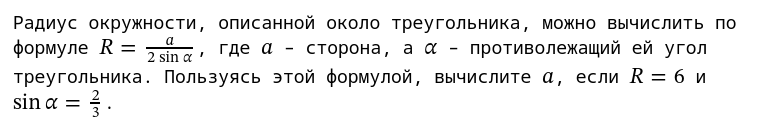
\includegraphics[width=1.4\textwidth]{506300-4-2.png}
